\section{Pixels, Perception, and the Problem of Meaning}

We begin with an image.  
An image is, at its most fundamental level, a grid—an ordered arrangement of pixels, each encoded as a numerical value representing color intensity or brightness. This numerical structure is the raw material of vision, both for biological and artificial systems.

But this raises a fundamental question:  
\textit{Do these pixels carry meaning?}

Philosophically, we must be careful. It is tempting to assume that because an image depicts something—say, a cat, a crack, or a defect—that its pixels ``contain'' that meaning. But this is a projection. Pixels, in isolation, are \textit{raw information}. They may \textit{reflect structure}—like the contours of an edge or the repetition of texture—but they do not carry meaning in the way that a concept or label does. The image may encode structure, patterns, even hints of semantic content—but that content is \textit{not explicit}, and it is certainly \textit{not accessible on its own}. Meaning is not embedded in the numbers; it arises through a \textit{relationship between those numbers and a system capable of interpreting them}.

Consider a single pixel with a value of 240.  
What does that number signify? By itself: nothing.  
It is only in the context of neighboring pixels, and within the interpretive framework of a model or a mind, that this number becomes part of an edge, a shadow, or an object.

Thus, we must distinguish carefully:
\begin{itemize}
	\item \textbf{The image may contain structure}—regularities, symmetries, contrasts.
	\item \textbf{It may point toward meaning}.
	\item But it \textbf{does not express that meaning directly}.
\end{itemize}

\begin{quote}
	The pixels hold the potential for meaning, but not the meaning itself.  
	That meaning must be uncovered, constructed, or interpreted by a system trained to recognize it.
\end{quote}

In deep learning, that system is the model—a network of transformations designed to take raw pixels and transform them, step by step, into something usable, expressive, and aligned with a specific task. But the model cannot skip ahead. It must begin in the pixel space—with no assumptions, no built-in knowledge—and learn how to carve meaning from numerical arrangement.

\section{Vectors as Movements in Space}

Before we understand linear transformations, we must understand what they transform: vectors. A vector is more than just an ordered list of numbers—it is a \textit{movement}, a \textit{displacement}, a \textit{directional quantity}.

Consider the vector \( \vec{v} = \begin{bmatrix} 3 \\ 2 \end{bmatrix} \). This can be interpreted as an instruction: start at the origin \( (0, 0) \), move 3 units to the right (along the x-axis), and then 2 units upward (along the y-axis). The result is a new position: the point \( (3, 2) \).

\begin{center}
	\textit{A vector is a directed arrow from one point to another, typically drawn from the origin.}
\end{center}

Vectors can be \textbf{added}, which corresponds to chaining movements, and they can be \textbf{scaled}, which changes the magnitude (length) of the movement without changing its direction.

\subsection*{Vector Addition}
Given two vectors:
\[
\vec{a} = \begin{bmatrix} 1 \\ 2 \end{bmatrix}, \quad
\vec{b} = \begin{bmatrix} 3 \\ 1 \end{bmatrix}
\]
Their sum is:
\[
\vec{a} + \vec{b} = \begin{bmatrix} 4 \\ 3 \end{bmatrix}
\]
This corresponds to placing the tail of \( \vec{b} \) at the head of \( \vec{a} \), forming the diagonal of a parallelogram.

\subsection*{Scalar Multiplication}
Scaling a vector by a number stretches or shrinks it. For example:
\[
2 \vec{v} = 2 \begin{bmatrix} 3 \\ 2 \end{bmatrix} = \begin{bmatrix} 6 \\ 4 \end{bmatrix}
\]
This is a movement in the same direction as \( \vec{v} \), but twice as long. To better visualize these operations, consider the following illustrations. Each shows a different fundamental vector operation.


% Inside your document
\begin{figure}[h!]
	\centering
	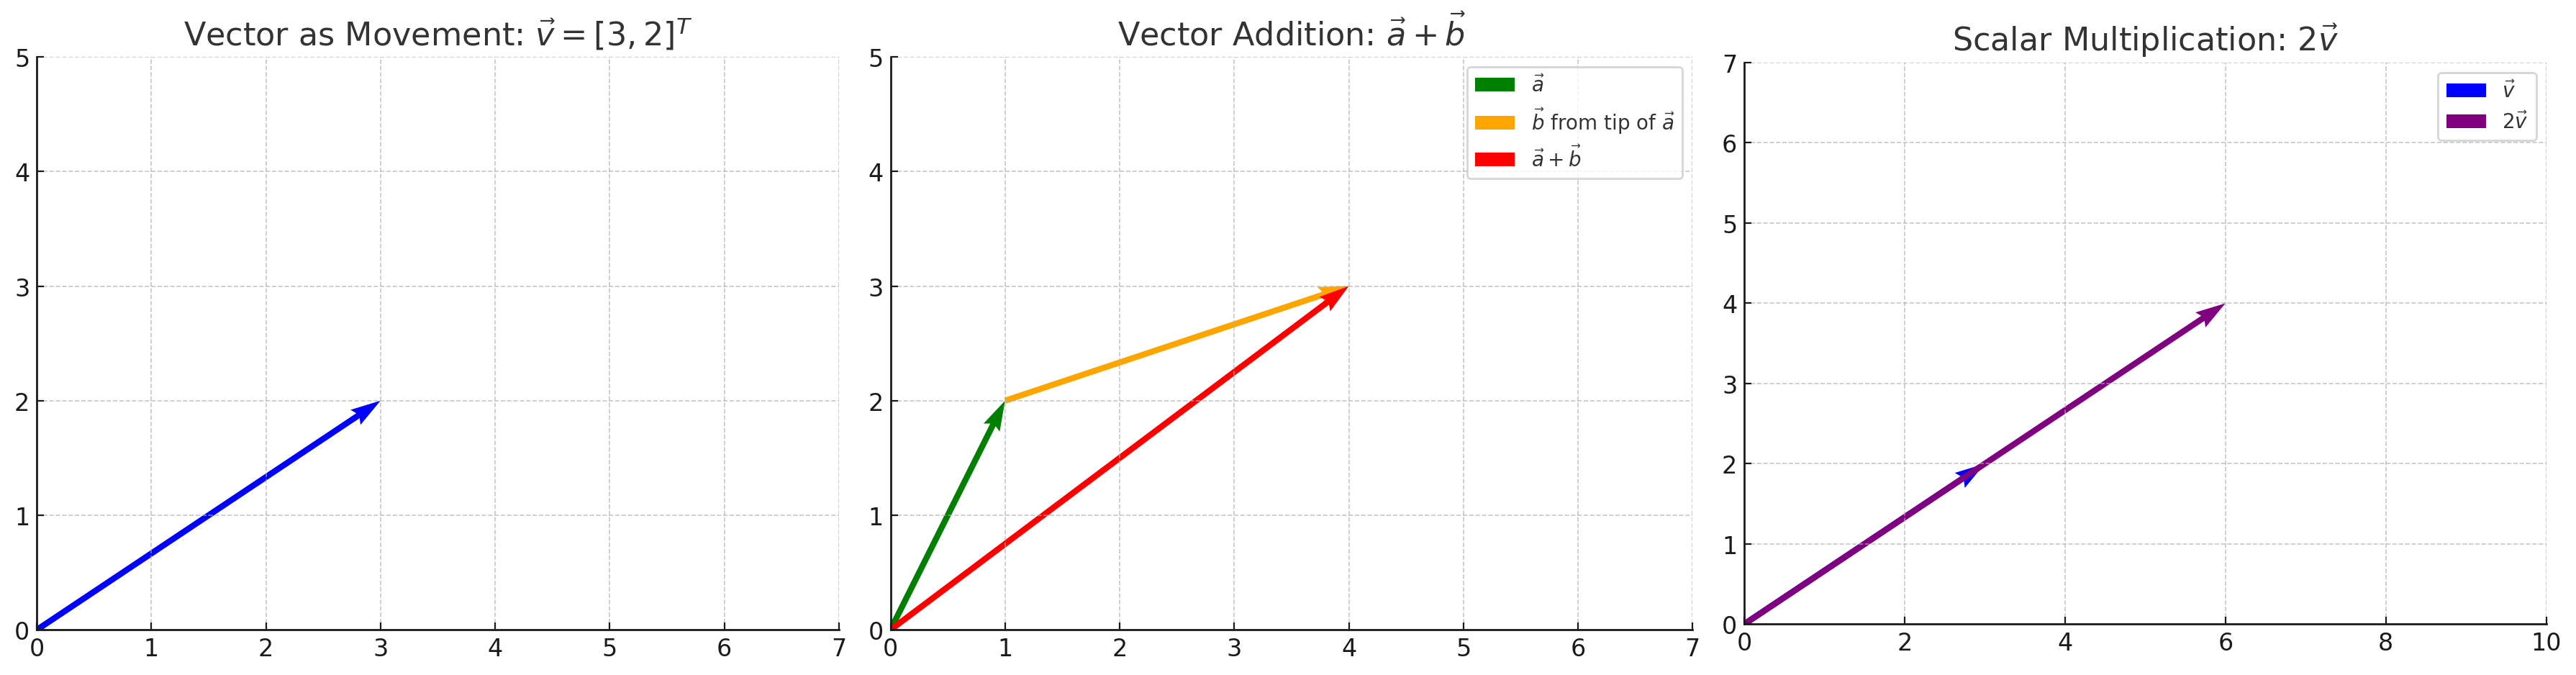
\includegraphics[width=\textwidth]{figures/vector_addition_multiplication.png}
	\caption{Visualizing vector movement, addition, and scalar multiplication.}
	\label{fig:vector_basics}
\end{figure}

Understanding vectors as movements in space lays the geometric foundation for understanding how they can be transformed, reshaped, and reoriented using linear transformations.

\section{The Philosophical Necessity of Linear Transformation in Image Processing}

To perceive is to transform. The world does not offer itself in neatly labeled form—it presents patterns, textures, and arrangements. To recognize structure within raw data, a system must transform it. In deep learning, particularly in image processing, this transformation begins with a fundamental operation: the \textit{linear transformation}.

An image, at its core, is a grid of intensity values—nothing more than an ordered collection of numbers. However, these values in their raw form do not convey structure or meaning. They must be reinterpreted. A linear transformation provides the means to do so.

\begin{definition}
	A linear transformation is a function \( T: \mathbb{R}^n \rightarrow \mathbb{R}^m \) that satisfies the following properties:
	\begin{align*}
		T(\mathbf{a} + \mathbf{b}) &= T(\mathbf{a}) + T(\mathbf{b}) \\
		T(c \cdot \mathbf{a}) &= c \cdot T(\mathbf{a})
	\end{align*}
\end{definition}

In other words, it respects the structure of the space—it preserves addition and scalar multiplication. Philosophically, this is vital: a linear transformation does not distort relationships arbitrarily; it reshapes space while maintaining consistency. It can stretch, rotate, reflect, or project—but it never bends.

In image processing, an image of dimension \( 28 \times 28 \) can be flattened into a vector in \( \mathbb{R}^{784} \). Passing this vector through a linear transformation reshapes it into a new space, potentially revealing latent patterns not apparent in the original pixel arrangement. This process is not simply numerical—it is perceptual. It reorients the data to make meaningful structures easier to extract.

\[
\mathbf{y} = A\mathbf{x}
\]

Here, \( \mathbf{x} \in \mathbb{R}^{n} \) is the input image vector, \( A \in \mathbb{R}^{m \times n} \) is the transformation matrix (learned in neural networks), and \( \mathbf{y} \in \mathbb{R}^m \) is the transformed representation.

\textit{Linear transformations do not merely shift numbers—they shift perspectives. They give a model the ability to perceive form within chaos.}



\section{Matrices Support Transformation}

\textit{At the heart of deep learning is the idea to learn from change.}  
This is not a poetic abstraction—it is a foundational truth. One of the many dimensions of Learning is the recognition that \textit{something is no longer the same as it was}. Whether in a biological mind or an artificial network, learning does not arise from repetition. For example, if a person is repeatedly making the same mistake then we can say that the person is not learning. Therefore, learning comes from \textit{difference}.

In the world of deep learning, we develop and train models that can make accurate predictions in the task that they have been developed and trained. During training stage, when a model makes an incorrect prediction, the misalignment between output and ground truth becomes the source of learning. It is not the prediction alone that teaches, nor the data alone—but the \textit{discrepancy} between the two. In other words, change is not an accident—it is the \textit{signal}. However, recognizing change is not enough. To learn from it, the system must represent it, measure it, and respond to it in a structured way. When we say a system must “represent” change, we are saying:
\begin{itemize}
	\item It must hold in memory some version of what has changed.
	\item It must structure that memory so that learning becomes possible.
\end{itemize}

So this representation must contain:
\begin{itemize}
	\item What is being changed (the values),
	\item How those values relate to others around them (the structure or pattern of change).
\end{itemize}

Learning doesn’t occur on values alone—it occurs on patterns in how those values interact. Imagine two examples:
\begin{itemize}
	\item If one pixel in an image becomes brighter, that’s a \textit{local} change.
	\item But if the whole region changes from “a cat” to “a dog,” that’s a \textit{structural} or \textit{relational} change.
\end{itemize}
To understand that, the model must not just know \textit{what} changed (value), but also:
\begin{itemize}
	\item Where it changed
	\item In relation to what
	\item How far that change propagates
\end{itemize}
So relationships matter: they tell us how changes in one place affect meaning in context and a Matrix help us Encode this.  

A matrix is a grid of numbers. But critically:
\begin{itemize}
	\item Each number (value) sits in a position (row, column).
	\item This position gives context: it tells us which values are near, which are far, and what kind of structure exists.
\end{itemize}

\textbf{Example:}
\[
\begin{bmatrix}
	5 & 5 & 5 \\
	5 & 10 & 5 \\
	5 & 5 & 5 \\
\end{bmatrix}
\]
Here, “10” is a value, but it's only meaningful because it’s surrounded by 5s.  
The matrix lets us perceive that the center stands out—this is a relational insight. So the matrix doesn't just store the value “10”, but also the fact that “10 is central, different, and structurally significant.” This structured way requires a data format that:
\begin{itemize}
	\item Stores values (what changed)
	\item Preserves relationships (how values relate across space or time)
\end{itemize}
This demands a form that can express both \textit{values and relationships}, a format that preserves the \textit{geometry of information}. That form is the \textbf{matrix}.Matrix doesn’t just hold numbers; it holds them \textit{in relation to one another}, giving us:
\begin{itemize}
	\item Local patterns
	\item Global structure
	\item The ability to transform both using algebra
\end{itemize}
Without matrices, the model would only have isolated data. With matrices, it can reason about form, flow, and pattern. A matrix is more than a table of numbers. It is a space in which \textit{relationships are embedded directly into structure}—where each element is not isolated but defined partly by its position. In image data, for instance, nearby pixels often carry related meaning; a matrix preserves this locality. In networks, weight matrices store learned transformations that map inputs to outputs—not just pointwise, but as \textit{global patterns of change}.

Moreover, the very act of learning—mathematically speaking—is guided by gradients, which are formal expressions of \textit{how a change in one value affects change in another}. These gradients are computed using \textit{matrix calculus}, and applied as updates to other matrices—weights, activations, filters. In this sense, matrices are not merely passive containers; they are the \textit{medium through which change flows and accumulates}.
\begin{quote}
	Learning from change requires more than memory. It requires a form that supports structured transformation. The matrix is that form—it both holds and evolves information, enabling the system to encode not only what \textit{is}, but how what \textit{is} can become something more.
\end{quote}

\section{Controlled Transformations}

\textit{To learn is not merely to observe change—it is to shape it.}  
A machine learning system does not passively witness variation; it seeks to modify its internal state in response to that variation, aiming to reduce error, increase accuracy, and discover structure. But such modification must be \textit{disciplined}, not random. Learning is effective only when the transformations it performs are \textbf{controlled}—that is, intentional, measurable, and adjustable.

In deep learning, transformation refers to the process by which one representation is mapped into another. This mapping is typically achieved through \textit{matrix multiplication}, where an input (such as a vector or a matrix) is multiplied by a weight matrix to produce a new form. But unlike traditional systems with fixed rules, deep learning models \textit{learn} the parameters of these transformations. The model does not begin with knowledge of how inputs should be transformed—it discovers those transformations over time, guided by a signal: the \textbf{gradient}.

The gradient provides the essential mechanism of control. It measures how small changes in each parameter affect the final error. Using this information, the model adjusts its transformation matrices to move toward lower error. This process—\textit{gradient descent}—is repeated iteratively, causing the system to slowly refine the structure of its transformations. In this sense, the matrix is not a static operator; it is a \textit{learnable transformation function}, evolving with experience.

This notion of control is crucial. If transformations were random or fixed, the system could not adapt to new data or improve from failure. What makes learning possible is the fact that transformation is \textit{both structured and malleable}. The matrix gives us the structure; the gradient gives us the malleability.

\begin{quote}
	In this view, learning becomes the art of discovering how to transform one state of representation into another—not by chance, but by adjusting internal transformations under the discipline of feedback. The matrix is the medium. The gradient is the guide. And the transformation is the soul of learning.
\end{quote}

\section{The Philosophy of Composition}

\textit{Complex understanding begins with simple parts.}  
This principle is not exclusive to deep learning; it is a general law of cognition, perception, and language. Our minds are structured to interpret the world not as a chaos of unrelated facts, but as \textit{systems of nested relationships}—layers of meaning that emerge from simpler building blocks.

In language, individual sounds form syllables, which become words. Words combine into phrases, and phrases into arguments. In vision, pixels form edges, edges form shapes, and shapes form objects. This compositional logic is not superficial—it is foundational. We do not merely observe the world; we build its meaning piece by piece.

Deep learning mirrors this process through architecture. A neural network does not attempt to leap from raw data to abstract conclusions in a single step. Instead, it applies a sequence of transformations—each layer refining, amplifying, or reorganizing what came before. These layers do not operate in isolation; they are \textit{composed}, meaning each one \textit{receives, modifies, and passes on} the work of the previous.

What emerges is a \textbf{hierarchy of representation}. The lower layers capture fine detail and local structure. Middle layers begin to recognize combinations and patterns. Higher layers abstract away from the specifics to form conceptual categories. But this ascent in abstraction is only possible because of \textbf{composition}—the deliberate layering of small, learnable transformations into a coherent whole.

\begin{quote}
	Composition is the scaffold of meaning. Without it, learning would remain flat and disconnected. With it, the system gains depth—not just in architecture, but in insight.
\end{quote}

\subsection{Why Convolutional Kernels Have Shape}

It is only in the context of neighboring pixels, and within the interpretive framework of a model or a mind, that any individual pixel becomes meaningful—whether as part of an edge, a shadow, or an object. A single pixel by itself does not represent structure; it must be situated within a surrounding region that reveals contrast, orientation, or spatial configuration.

This is precisely why convolutional kernels are designed with specific height and width.  
The kernel defines the \textit{local region of context} that the model will use to interpret the presence or absence of a pattern. By sliding this kernel across the image, the model is essentially asking, repeatedly:
\begin{quote}
	“Does this arrangement of pixels match a structure I’ve learned to recognize?”
\end{quote}

The choice of kernel size is not arbitrary—it encodes an assumption about \textit{how much context is necessary} to extract meaningful relationships. A $3 \times 3$ kernel captures very local structures, such as edges or corners. A $5 \times 5$ or larger kernel can capture more extended features—such as curves, textures, or small motifs. If the kernel is too small, it may miss global coherence; if too large, it may dilute local detail.

In this sense, the kernel is a kind of \textbf{window of perception}: it frames the portion of the visual field that the model is allowed to consider at once. The size of this window determines the \textit{scale of patterns} the model is capable of detecting. A kernel is therefore both a computational tool and a philosophical commitment—it defines what constitutes a “pattern” in the world, and how far the model must look to find one.


\section{Images as Structured Tensors}

In the context of deep learning, an image is not merely a visual representation but a structured numerical object—a tensor with defined dimensions and meaning. Mathematically, an image is represented as a three-dimensional tensor \( \mathbb{R}^{C \times H \times W} \), where \( C \) denotes the number of color channels (e.g., 3 for RGB), and \( H \) and \( W \) refer to the image’s height and width in pixels. When processed in batches during training, this tensor extends to four dimensions \( \mathbb{R}^{N \times C \times H \times W} \), with \( N \) representing the batch size. This format is standard in frameworks like PyTorch, while TensorFlow typically adopts the \( N \times H \times W \times C \) layout. 

Despite their numerical structure, these pixel values—intensities normalized between 0 and 1 or rescaled—carry no inherent semantic content. A value such as 182, for instance, is just a scalar unless it is interpreted within a channel and spatial configuration. The convolutional layer receives this tensor and treats it as a raw signal. It is not the pixel values in isolation but rather their arrangement and proximity that lay the groundwork for meaningful interpretation. Thus, even before learning begins, the architecture presumes that information is spatially organized, and that meaning—if any—is embedded in relationships, not in individual values.

\begin{lstlisting}[caption=Creating and passing an image through a Conv2d layer in PyTorch]
	import torch
	
	# A batch of 1 image, with 3 channels, 32x32 pixels
	image = torch.randn(1, 3, 32, 32)
	
	import torch.nn as nn
	conv = nn.Conv2d(in_channels=3, out_channels=16, kernel_size=3, padding=1)
	output = conv(image)
\end{lstlisting}

\begin{lstlisting}[caption=Creating and passing an image through a Conv2D layer in TensorFlow]
	import tensorflow as tf
	
	# A batch of 1 image, shape: (batch_size, height, width, channels)
	image = tf.random.normal([1, 32, 32, 3])
	
	conv = tf.keras.layers.Conv2D(filters=16, kernel_size=3, padding='same')
	output = conv(image)
\end{lstlisting}


\section{Contextualizing Semantic Meaning}

The notion of "meaning" in data processing, particularly in deep learning, requires careful qualification. A single numerical value—such as a pixel intensity—does not possess semantic significance on its own. To understand this more precisely, it is helpful to distinguish between structural, syntactic, and semantic meaning. \textbf{Structural information} refers to how elements are arranged—for example, the shape of a matrix or the order of words in a sentence. In an image, this could correspond to the layout of pixel rows and columns. \textbf{Syntactic information}, in turn, involves formal rules that govern how elements can be combined. For instance, in programming, syntax dictates how variables and operations can be combined legally; in language, it tells us that a sentence must have a subject and a verb. These structural and syntactic patterns define form, but not content.

\paragraph{Example of Structural Information.}
In natural language, structural information refers to the order of words. For instance, the two sentences:
\begin{quote}
	\textit{``The cat chased the mouse.''} \\
	\textit{``The mouse chased the cat.''}
\end{quote}
contain the same words and obey grammatical rules, but their structure leads to entirely different interpretations due to the changed positions of subject and object.

In image data, structure corresponds to the spatial arrangement of pixels. For example, a 3$\times$3 matrix of pixel values like:
\[
\begin{bmatrix}
	100 & 100 & 100 \\
	0 & 0 & 0 \\
	100 & 100 & 100 \\
\end{bmatrix}
\]
may suggest a horizontal edge due to the contrast between rows, a pattern that would not exist if the same values were shuffled randomly.

\paragraph{Example of Syntactic Information.}
In programming languages, syntax dictates how symbols must be arranged. The expression:
\begin{quote}
	\texttt{int x = 5;}
\end{quote}
is syntactically correct in C++, whereas:
\begin{quote}
	\texttt{int = x 5;}
\end{quote}
is not, even though it uses the same tokens. The syntax defines which forms are valid, not what the variables or values represent.

In deep learning, syntactic rules may refer to tensor compatibility. For example, attempting to multiply a tensor of shape $(3 \times 4)$ with a tensor of shape $(5 \times 6)$ will result in an error, not because of semantic issues, but because the operation is syntactically invalid under matrix multiplication rules.


\textbf{Semantic meaning}, on the other hand, pertains to what something \emph{refers to} or \emph{implies} in a given context. In natural language, the word “bank” has different semantic interpretations depending on context—it may refer to a financial institution or the edge of a river. Similarly, in an image, a pixel value of 182 in the red channel is just a number unless it is part of a spatial pattern that may represent, for instance, the curvature of a handwritten digit or the contour of a car. In convolutional networks, it is not the absolute values of pixels that carry semantic weight but their patterns of co-occurrence across space and channels. These relationships make it possible for a model to infer edges, textures, and object parts—not because any single pixel is meaningful, but because groups of pixels form structures that align with higher-level concepts. Hence, semantics are not properties of isolated numbers but emerge through structured, relational interpretation.

\section{The Role of the Convolutional Layer}

A convolutional layer is a fundamental building block in deep learning models for processing spatially structured data such as images. It operates by sliding a set of small filters, or kernels, over the input tensor to produce feature maps that capture local patterns. Each filter performs a dot product between its weights and a local patch of the input, effectively highlighting specific types of local variation. However, at initialization, these filters are randomly assigned and have no prior knowledge of what constitutes a meaningful feature. The convolution operation itself encodes only a structural prior: the assumption that useful information is often localized and translationally invariant. It provides a mechanism for detecting patterns, but not for determining which patterns are significant.

The filters gain semantic relevance only through training. As data is passed through the network and predictions are compared to known targets, feedback in the form of gradients adjusts the weights of the filters. Over time, this process causes the filters to specialize in detecting features that are useful for the task—such as edges, textures, and object parts. The key insight here is that convolutional layers do not explicitly extract semantic features because they have been told what to look for; rather, they extract features that emerge as semantically meaningful because they help reduce the model’s error. Thus, the role of the convolutional layer is not to encode meaning directly, but to provide a structured interface through which meaningful patterns can be discovered via optimization.

\begin{lstlisting}[caption=Training a convolutional layer: random initialization and learning via gradient descent]
	import torch
	import torch.nn as nn
	import torch.optim as optim
	
	# Define a simple Conv2D layer followed by flattening and linear output
	conv = nn.Conv2d(in_channels=3, out_channels=2, kernel_size=3, padding=1)
	linear = nn.Linear(2 * 32 * 32, 10)  # e.g., 10-class classification
	
	# Combine into a simple model
	model = nn.Sequential(conv, nn.Flatten(), linear)
	
	# Dummy image and label
	image = torch.randn(1, 3, 32, 32)         # input image
	target = torch.randint(0, 10, (1,))       # random class label
	
	# Define loss and optimizer
	criterion = nn.CrossEntropyLoss()
	optimizer = optim.SGD(model.parameters(), lr=0.01)
	
	# Forward pass
	output = model(image)
	loss = criterion(output, target)
	
	# Backward pass and update
	optimizer.zero_grad()
	loss.backward()
	optimizer.step()
\end{lstlisting}

\section{Emergence of Semantics Through Optimization}

The ability of neural networks to extract semantically meaningful features does not arise from the mechanics of convolution or gradient descent alone. Gradient descent is a purely numerical procedure; it does not encode domain knowledge or interpretative goals. Its function is to iteratively minimize a loss function by adjusting the model's weights in response to observed errors. As such, it responds only to whether a prediction is closer to or further from a desired target. The semantic orientation of the features—such as whether a learned filter detects an eye, an edge, or a tail—is not embedded in the algorithm, but is a consequence of the \emph{structure} of the task. Specifically, the loss function, paired with labeled data, defines what counts as success. This definition then drives the network to prioritize features that improve performance on that task.

As training progresses, features that consistently help reduce loss are reinforced, while uninformative features are suppressed. In this way, filters gradually specialize—not due to an explicit semantic signal, but because semantic features tend to be functionally useful in minimizing task-specific error. For example, in a dog-vs-cat classifier, filters that respond to fur texture, ear shape, or eye placement become statistically favorable because they help differentiate between the two classes. These features \emph{acquire} semantic meaning as a side effect of being useful. Therefore, the emergence of semantics is not the result of direct supervision on meaning itself, but rather of a system that, through task performance, converges on patterns that align with meaningful structure in the data.

\begin{lstlisting}[caption=Semantics emerge from loss-driven adaptation rather than explicit supervision]
	import torch
	import torch.nn as nn
	import torch.optim as optim
	
	# A small CNN for binary classification (e.g., cat vs dog)
	class SmallCNN(nn.Module):
	def __init__(self):
	super().__init__()
	self.conv = nn.Conv2d(3, 8, 3, padding=1)  # 8 random filters
	self.pool = nn.AdaptiveAvgPool2d((1, 1))
	self.fc = nn.Linear(8, 2)  # Binary classifier
	
	def forward(self, x):
	x = torch.relu(self.conv(x))  # Learn features via ReLU
	x = self.pool(x).view(x.size(0), -1)
	return self.fc(x)
	
	model = SmallCNN()
	optimizer = optim.Adam(model.parameters(), lr=0.001)
	criterion = nn.CrossEntropyLoss()
	
	# Training step (simulated)
	image = torch.randn(1, 3, 64, 64)               # Input image
	label = torch.tensor([1])                      # Target class: e.g., "dog"
	
	# Forward, backward, update
	output = model(image)
	loss = criterion(output, label)
	optimizer.zero_grad()
	loss.backward()
	optimizer.step()
\end{lstlisting}


